\section{Teilversuch 1: Vermessung des Magnetfeldes}
	Fehler $\Delta B = \pm \SI{10}{\milli\tesla}$
	\begin{center}
		\begin{tabular}{l | *{10}{r}}
			\toprule
			$I/\si{\ampere}$ & \num{1.070} & \num{2.096} & \num{2.995} & \num{4.153} & \num{5.300} & \num{6.033} & \num{7.09} & \num{8.03} & \num{9.06} & \num{9.48} \\
			$\Delta I/\si{\ampere}$ & \num{0.005} & \num{0.005} & \num{0.010} & \num{0.020} & \num{0.010} & \num{0.010} & \num{0.01} & \num{0.01} & \num{0.01} & \num{0.01} \\
			\midrule
			$B/\si{\milli\tesla}$ & \num{671} & \num{1298} & \num{1910} & \num{2700} & \num{3460} & \num{3950} & \num{4630} & \num{5240} & \num{5750} & \num{5970} \\
			\bottomrule
		\end{tabular}
	\end{center}
	Als Hintergrund haben wir zwei Messungen:
	\begin{center}
		\begin{tabular}{ll}
			\toprule
			Messung & Hintergrund \\
			\midrule
			Davor  & \SI{0.11(2)}{\milli\tesla} \\
			Danach & \SI{1.13(2)}{\milli\tesla} \\
			\bottomrule
		\end{tabular}
	\end{center}
	Da diese Hintergrundwerte deutlich unter der Unsicherheit $\Delta B$ liegt, vernächlässigen wir den Hintergrund. 
	\newpage
	Wir führen nun eine Kurveanpassung zu $B = mI + c$ mittels \gnuplot{} durch (siehe Appendix \ref{appdx:tv1}):
	\begin{figure}[!ht]
		\vspace{-1em}
	    \centering
	    % GNUPLOT: LaTeX picture with Postscript
\begingroup
  \makeatletter
  \providecommand\color[2][]{%
    \GenericError{(gnuplot) \space\space\space\@spaces}{%
      Package color not loaded in conjunction with
      terminal option `colourtext'%
    }{See the gnuplot documentation for explanation.%
    }{Either use 'blacktext' in gnuplot or load the package
      color.sty in LaTeX.}%
    \renewcommand\color[2][]{}%
  }%
  \providecommand\includegraphics[2][]{%
    \GenericError{(gnuplot) \space\space\space\@spaces}{%
      Package graphicx or graphics not loaded%
    }{See the gnuplot documentation for explanation.%
    }{The gnuplot epslatex terminal needs graphicx.sty or graphics.sty.}%
    \renewcommand\includegraphics[2][]{}%
  }%
  \providecommand\rotatebox[2]{#2}%
  \@ifundefined{ifGPcolor}{%
    \newif\ifGPcolor
    \GPcolortrue
  }{}%
  \@ifundefined{ifGPblacktext}{%
    \newif\ifGPblacktext
    \GPblacktexttrue
  }{}%
  % define a \g@addto@macro without @ in the name:
  \let\gplgaddtomacro\g@addto@macro
  % define empty templates for all commands taking text:
  \gdef\gplbacktext{}%
  \gdef\gplfronttext{}%
  \makeatother
  \ifGPblacktext
    % no textcolor at all
    \def\colorrgb#1{}%
    \def\colorgray#1{}%
  \else
    % gray or color?
    \ifGPcolor
      \def\colorrgb#1{\color[rgb]{#1}}%
      \def\colorgray#1{\color[gray]{#1}}%
      \expandafter\def\csname LTw\endcsname{\color{white}}%
      \expandafter\def\csname LTb\endcsname{\color{black}}%
      \expandafter\def\csname LTa\endcsname{\color{black}}%
      \expandafter\def\csname LT0\endcsname{\color[rgb]{1,0,0}}%
      \expandafter\def\csname LT1\endcsname{\color[rgb]{0,1,0}}%
      \expandafter\def\csname LT2\endcsname{\color[rgb]{0,0,1}}%
      \expandafter\def\csname LT3\endcsname{\color[rgb]{1,0,1}}%
      \expandafter\def\csname LT4\endcsname{\color[rgb]{0,1,1}}%
      \expandafter\def\csname LT5\endcsname{\color[rgb]{1,1,0}}%
      \expandafter\def\csname LT6\endcsname{\color[rgb]{0,0,0}}%
      \expandafter\def\csname LT7\endcsname{\color[rgb]{1,0.3,0}}%
      \expandafter\def\csname LT8\endcsname{\color[rgb]{0.5,0.5,0.5}}%
    \else
      % gray
      \def\colorrgb#1{\color{black}}%
      \def\colorgray#1{\color[gray]{#1}}%
      \expandafter\def\csname LTw\endcsname{\color{white}}%
      \expandafter\def\csname LTb\endcsname{\color{black}}%
      \expandafter\def\csname LTa\endcsname{\color{black}}%
      \expandafter\def\csname LT0\endcsname{\color{black}}%
      \expandafter\def\csname LT1\endcsname{\color{black}}%
      \expandafter\def\csname LT2\endcsname{\color{black}}%
      \expandafter\def\csname LT3\endcsname{\color{black}}%
      \expandafter\def\csname LT4\endcsname{\color{black}}%
      \expandafter\def\csname LT5\endcsname{\color{black}}%
      \expandafter\def\csname LT6\endcsname{\color{black}}%
      \expandafter\def\csname LT7\endcsname{\color{black}}%
      \expandafter\def\csname LT8\endcsname{\color{black}}%
    \fi
  \fi
    \setlength{\unitlength}{0.0500bp}%
    \ifx\gptboxheight\undefined%
      \newlength{\gptboxheight}%
      \newlength{\gptboxwidth}%
      \newsavebox{\gptboxtext}%
    \fi%
    \setlength{\fboxrule}{0.5pt}%
    \setlength{\fboxsep}{1pt}%
    \definecolor{tbcol}{rgb}{1,1,1}%
\begin{picture}(8640.00,5760.00)%
    \gplgaddtomacro\gplbacktext{%
      \csname LTb\endcsname%%
      \put(946,704){\makebox(0,0)[r]{\strut{}$0$}}%
      \put(946,1332){\makebox(0,0)[r]{\strut{}$1000$}}%
      \put(946,1960){\makebox(0,0)[r]{\strut{}$2000$}}%
      \put(946,2588){\makebox(0,0)[r]{\strut{}$3000$}}%
      \put(946,3215){\makebox(0,0)[r]{\strut{}$4000$}}%
      \put(946,3843){\makebox(0,0)[r]{\strut{}$5000$}}%
      \put(946,4471){\makebox(0,0)[r]{\strut{}$6000$}}%
      \put(946,5099){\makebox(0,0)[r]{\strut{}$7000$}}%
      \put(1078,484){\makebox(0,0){\strut{}$0$}}%
      \put(2511,484){\makebox(0,0){\strut{}$2$}}%
      \put(3944,484){\makebox(0,0){\strut{}$4$}}%
      \put(5377,484){\makebox(0,0){\strut{}$6$}}%
      \put(6810,484){\makebox(0,0){\strut{}$8$}}%
      \put(8243,484){\makebox(0,0){\strut{}$10$}}%
    }%
    \gplgaddtomacro\gplfronttext{%
      \csname LTb\endcsname%%
      \put(209,2901){\rotatebox{-270}{\makebox(0,0){\strut{}Magnetfeldstärke $B$ ($\si{\milli\tesla}$)}}}%
      \put(4660,154){\makebox(0,0){\strut{}Strom $I$ ($\si{\ampere}$)}}%
      \csname LTb\endcsname%%
      \put(7256,1427){\makebox(0,0)[r]{\strut{}$(641,75932)I + (5,09225)$}}%
      \csname LTb\endcsname%%
      \put(7256,987){\makebox(0,0)[r]{\strut{}Messpunkte}}%
      \csname LTb\endcsname%%
      \put(4660,5429){\makebox(0,0){\strut{}Magnetfeldstärke $B$ gegen Strom $I$}}%
    }%
    \gplbacktext
    \put(0,0){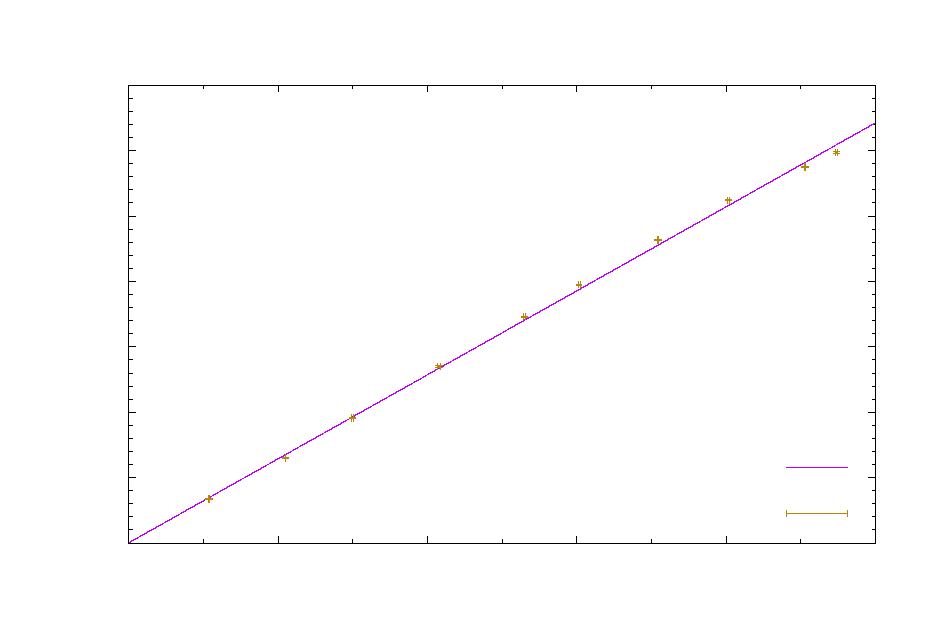
\includegraphics[width={432.00bp},height={288.00bp}]{tv1}}%
    \gplfronttext
  \end{picture}%
\endgroup

	    \caption{\centering Magnetfeldstärke gegen Strom $\left(\chi^2_{\text{red}} = \num{39.1889} \text{ (klein gegen Werten)} \Rightarrow \text{Gute Anpassung}\right)$}
	    \label{fig:tv1}
	    \vspace{-1em}
	\end{figure}

	Als Endergebnis erhalten wir:
	\begin{center}
		\begin{tabular}{lll}
			\toprule
			Variable & Roh & Gerundet \\
			\midrule
			$m$ 
				& \SI{641.759(8077)}{\milli\tesla\per\ampere} 
				& \SI{641(9)}{\milli\tesla\per\ampere} \\
			$c$ 
				& \SI{5.09(4933)}{\milli\tesla} 
				& \SI{5(50)}{\milli\tesla}  \\
			\bottomrule
		\end{tabular}
	\end{center}
	Da $0$ im Fehlerintervall von $c$ liegt, ist die Kurveanpassung auch vernünftig. Für die Kalibrierung von Strom zu Magnetfeldstärke dient also die folgende Formel:
	\begin{align}
		B / \si{\milli\tesla} &= 641 \times I + 5 \\
		\Delta B / \si{\milli\tesla} &= \gausserror{B}{m,I,c} \notag \\
		&= \sqrt{\left(I\Delta m\right)^2 + (m\Delta I)^2 + \left(\Delta c\right)^2} \notag \\
		&= \sqrt{81I^2 + 410881(\Delta I)^2 + 2500}
	\end{align}